\documentclass[compress,usepdftitle=false]{beamer}

\usepackage{catchfile}
\usepackage{ifthen}
\CatchFileDef\TheLanguage{../language.tex}{\endlinechar=-1}
\ifthenelse{\equal{\TheLanguage}{french}}
 {
  \usepackage[french]{babel}
 }
 {
  \usepackage[english]{babel} 
 }
\usepackage[utf8]{inputenc}
\usepackage[T1]{fontenc}
\usepackage{amsmath,amssymb,amscd,amsthm}
\usepackage{latexsym}
\usepackage{eurosym}
%%%%%% FONT
\usepackage{libertine}
    %other font
    %\usepackage{times}
    %\usepackage{euscript}
    %\usepackage{avant}
    %\usepackage{mathptmx}
    %\usepackage{microtype}
    %\usepackage{bbm}
\usepackage{pifont}
\usepackage{graphicx}
%\usepackage{algorithmic}
%\usepackage{algorithm}
\usepackage{textpos}
\usepackage[normalem]{ulem}
\usepackage{tikz}
\usetikzlibrary{arrows.meta}
 \usetikzlibrary{automata,calc,shapes,mindmap,shadows,arrows,arrows.meta,patterns,matrix,positioning,snakes}
\usepackage{tikzsymbols}
\usepackage[all]{xy}
\usepackage{listings}
\usepackage{multirow}
\usepackage{array}
\usepackage{makecell}
\usepackage{hhline}
%\usepackage[framemethod=TikZ]{mdframed}
%\usepackage{diagbox}
\usepackage{stmaryrd}
\usepackage{fdsymbol}
\usepackage{colortbl}
\usepackage{catchfile}
\usepackage{ifthen}
\usepackage[lined,ruled,onelanguage,commentsnumbered,linesnumbered,inoutnumbered]{algorithm2e}
\usepackage{pgfplots}
\pgfplotsset{compat=1.9}
% We will externalize the figures
\usepgfplotslibrary{external}
%\tikzexternalize

\newcommand{\departementEPISEN}{SI}    % write SI or ITS or ISBS

%%%%%%%%%%%%%%%%%%%%%%%%%%%%%%%%%%%%%%%%%%%%%%%%%%%%%%%%%%%%%%%%%%%%%%%%%%
%%%%%%%%%%%%%%%%%%%%%%%%%%%%%%%%%%%%%%%%%%%%%%%%%%%%%%%%%%%%%%%%%%%%%%%%%%
%%%%%%%%%%%%%%%%%%%%%%%%%%%%%%%%%%%%%%%%%%%%%%%%%%%%%%%%%%%%%%%%%%%%%%%%%%
%%%%%%%%%%%%%%%%%%%%%%%%%%%%%%%%%%%%%%%%%%%%%%%%%%%%%%%%%%%%%%%%%%%%%%%%%%
%
%  A PRIORI, NE PAS MODIFIER CE FICHIER !
%
%%%%%%%%%%%%%%%%%%%%%%%%%%%%%%%%%%%%%%%%%%%%%%%%%%%%%%%%%%%%%%%%%%%%%%%%%%
%%%%%%%%%%%%%%%%%%%%%%%%%%%%%%%%%%%%%%%%%%%%%%%%%%%%%%%%%%%%%%%%%%%%%%%%%%
%%%%%%%%%%%%%%%%%%%%%%%%%%%%%%%%%%%%%%%%%%%%%%%%%%%%%%%%%%%%%%%%%%%%%%%%%%
%%%%%%%%%%%%%%%%%%%%%%%%%%%%%%%%%%%%%%%%%%%%%%%%%%%%%%%%%%%%%%%%%%%%%%%%%%


%%%%%%%%%%%%%%%%%%%%%%%%%%%%%%%%%%%%%%%%%%%%%%%%%%%%%%%%%%%%%%%%%%%%%%%%%%
%%%%%%%%%%%%%%%%%%%%%%%%%%%%%%%%%%%%%%%%%%%%%%%%%%%%%%%%%%%%%%%%%%%%%%%%%%
% *********************** LES COULEURS (Départements) ********************
%%%%%%%%%%%%%%%%%%%%%%%%%%%%%%%%%%%%%%%%%%%%%%%%%%%%%%%%%%%%%%%%%%%%%%%%%%
%%%%%%%%%%%%%%%%%%%%%%%%%%%%%%%%%%%%%%%%%%%%%%%%%%%%%%%%%%%%%%%%%%%%%%%%%%

\definecolor{linkEpisenGris}{RGB}{81 98 111}
\definecolor{colorEPISEN-UPEC}{HTML}{4c6172}
%\definecolor{cadmiumred}{rgb}{0.89, 0.0, 0.13}
\definecolor{redUPEC}{HTML}{ef293d}

\ifthenelse{\equal{\departementEPISEN}{ITS}}
  {
   %%%%%%%%%%%%%%%%%%%%%%%%%%% POUR ITS
   \definecolor{colorEPISEN-MEMOIRE}{HTML}{655aa0}
   \definecolor{linkEpisenMEMOIRE}{RGB}{101 90 160}
   \definecolor{linkEpisenPoster}{RGB}{101 90 160}
   %\definecolor{linkEpisenPosterLight}{RGB}{223 221 238}
   %\definecolor{linkEpisenPosterLight}{HTML}{dfddee}
   \colorlet{linkEpisenPosterLight}{linkEpisenPoster!20}
   \colorlet{linkEpisenMemoireUltraLight}{linkEpisenPoster!7}
  }
  {
   \ifthenelse{\equal{\departementEPISEN}{SI}}
    {
	%%%%%%%%%%%%%%%%%%%%%%%%%%% POUR SI
	\definecolor{colorEPISEN-MEMOIRE}{HTML}{009fe3}
	\definecolor{linkEpisenMEMOIRE}{RGB}{0 159 227}
	\definecolor{linkEpisenPoster}{RGB}{0 159 227}
	%\definecolor{linkEpisenPosterLight}{RGB}{204 239 252}
  %\definecolor{linkEpisenPosterLight}{HTML}{cceffc}
  \colorlet{linkEpisenPosterLight}{linkEpisenPoster!20}
  \colorlet{linkEpisenMemoireUltraLight}{linkEpisenPoster!7}
    }
    {
	%%%%%%%%%%%%%%%%%%%%%%%%%%% POUR ISBS
	\definecolor{colorEPISEN-MEMOIRE}{HTML}{2fac66}
	\definecolor{linkEpisenMEMOIRE}{RGB}{47 172 102}
	\definecolor{linkEpisenPoster}{RGB}{47 172 102}
  %\definecolor{linkEpisenPosterLight}{RGB}{217 241 225}
  %\definecolor{linkEpisenPosterLight}{HTML}{d9f1e1}
  \colorlet{linkEpisenPosterLight}{linkEpisenPoster!20}
  \colorlet{linkEpisenMemoireUltraLight}{linkEpisenPoster!7}
    }
  }


%\definecolor{linkEpisenCyan}{RGB}{0 159 227}
%\definecolor{linkEpisenVert}{RGB}{47 172 102}
%\definecolor{linkEpisenViolet}{RGB}{101 90 160}
%\definecolor{colorEPISEN-SI}{HTML}{009fe3}
%\definecolor{colorEPISEN-ISBS}{HTML}{2fac66}
%\definecolor{colorEPISEN-ITS}{HTML}{655aa0}
%\definecolor{colorEPISEN-UPEC}{HTML}{4c6172}



%%%%%%%%%%%%%%%%%%%%%%%%%%%%%%%%%%%%%%%%%%%%%%%%%%%%%%%%%%%%%%%%%%%%%%%%%%
%
%  VOUS POUVEZ APPORTER QUELQUES AJOUTS ICI
%
%%%%%%%%%%%%%%%%%%%%%%%%%%%%%%%%%%%%%%%%%%%%%%%%%%%%%%%%%%%%%%%%%%%%%%%%%%

%%%%%%%%%%%%%%%%%%%%%%%%%%%%%%%%%%%%%%%%%%%%%%%%%%%%%%%%%%%%%%%%%%%%%%%%%%
%%%%%%%%%%%%%%%%%%%%%%%%%%%%%%%%%%%%%%%%%%%%%%%%%%%%%%%%%%%%%%%%%%%%%%%%%%
%  Lecture des fichiers et données partagées
%%%%%%%%%%%%%%%%%%%%%%%%%%%%%%%%%%%%%%%%%%%%%%%%%%%%%%%%%%%%%%%%%%%%%%%%%%
%%%%%%%%%%%%%%%%%%%%%%%%%%%%%%%%%%%%%%%%%%%%%%%%%%%%%%%%%%%%%%%%%%%%%%%%%%
\CatchFileDef\TheManuscritTitle{../titre.tex}{\endlinechar=-1}
\CatchFileDef\TheAuthorEmail{../email.tex}{\endlinechar=-1}
\CatchFileDef\TheAuthorManuscript{../auteur.tex}{\endlinechar=-1}
\CatchFileDef\TheMemoireSubject{../sujet.tex}{\endlinechar=-1}
\CatchFileDef\TheMemoireKeywords{../keywords.tex}{\endlinechar=-1}

%%%%%%%%%%%%%%%%%%%%%%%%%%%%%%%%%%%%%%%%%%%%%%%%%%%%%%%%%%%%%%%%%%%%%%%%%%
%%% MODIFIER ICI POUR VOTRE PDF SI BESOIN
%%%%%%%%%%%%%%%%%%%%%%%%%%%%%%%%%%%%%%%%%%%%%%%%%%%%%%%%%%%%%%%%%%%%%%%%%%
\hypersetup{
  urlcolor=linkEpisenMEMOIRE,
  urlbordercolor=linkEpisenMEMOIRE,
  linkcolor=black,
  linkbordercolor=linkEpisenMEMOIRE,
  citecolor=linkEpisenMEMOIRE,
  citebordercolor=linkEpisenMEMOIRE,
  anchorcolor=linkEpisenMEMOIRE,
  pdftitle=\TheManuscritTitle,
  pdfauthor=\TheAuthorManuscript\\ (\TheAuthorEmail),
  pdfsubject=\TheMemoireSubject,
  pdfkeywords=\TheMemoireSubject
}


%%%%%%%%%%%%%%%%%%%%%%%%%%%%%%%%%%%%%%%%%%%%%%%%%%%%%%%%%%%%%%%%%%%%%%%%%%
%%% MODIFIER ICI pour les package tikz
%%%%%%%%%%%%%%%%%%%%%%%%%%%%%%%%%%%%%%%%%%%%%%%%%%%%%%%%%%%%%%%%%%%%%%%%%%
\usetikzlibrary{automata,positioning}
\AtBeginEnvironment{tikzpicture}{\tracinglostchars=0\relax}   % ==> pour éviter des warnings sur un nullfont


%%%%%%%%%%%%%%%%%%%%%%%%%%%%%%%%%%%%%%%%%%%%%%%%%%%%%%%%%%%%%%%%%%%%%%%%%%
%%% Programme
%%%%%%%%%%%%%%%%%%%%%%%%%%%%%%%%%%%%%%%%%%%%%%%%%%%%%%%%%%%%%%%%%%%%%%%%%%


%%% Java
%%%%%%%%%%%%%%%%%%%%%%%%%%%%%%%%%%%%%%%%%%%%%%%%%%%%%%%%%%%%%%%%%%%%%%%%%%
\lstdefinestyle{myJava}{language=java, 
  keywordstyle=\bfseries\color{black},
  basicstyle=\normalfont,
  commentstyle=\color{linkEpisenGris},
  stringstyle=\color{redUPEC},
   keepspaces=true, 
    numbers=left,
    numbersep=9pt,
    numberstyle=\tiny\color{linkEpisenGris},
    xleftmargin=20pt,
    framexleftmargin=1.77em,
    showstringspaces=true,
    showtabs=false,
    tabsize=2,
  breaklines=true,         % sets automatic line breaking
  breakatwhitespace=false, % sets if automatic breaks should only happen at whitespace
  columns=flexible,
  morekeywords={String, sealed, permits, System,out,println,-,+,*,/,++,--,<,>,=,!,!=},
  otherkeywords={\%*\%,+,!,!=,\&,<,>,=,++,--,\%/\%,\%\%},
  identifierstyle=\normalfont\itshape,
  literate=%
        {é}{{\'e}}1
        {è}{{\`e}}1
        {ê}{{\^e}}1
        {à}{{\`a}}1
        {â}{{\^a}}1
        {î}{{\^i}}1
        {ç}{{c}}1
        {ù}{{\`u}}1
      {|}{{$\hskip .001em\smash{\color{linkEpisenGris}\big|}\hskip .5em$}{ }}{1},
    mathescape=true,
}

\lstnewenvironment{java}
   {\lstset{style=myJava}}
   {}





%%% Python
%%%%%%%%%%%%%%%%%%%%%%%%%%%%%%%%%%%%%%%%%%%%%%%%%%%%%%%%%%%%%%%%%%%%%%%%%%

\lstdefinestyle{myPython}{language=python, 
  keywordstyle=\bfseries\color{black},
  basicstyle=\normalfont,
  commentstyle=\color{linkEpisenGris},
  stringstyle=\color{redUPEC},
    keepspaces=true, 
    numbers=left,
    numbersep=9pt,
    numberstyle=\tiny\color{linkEpisenGris},
    xleftmargin=20pt,
    framexleftmargin=1.5em,
    showstringspaces=true,
    showtabs=false,
    tabsize=2,
  breaklines=true,         % sets automatic line breaking
  breakatwhitespace=false, % sets if automatic breaks should only happen at whitespace
  columns=flexible,
  morekeywords={-,+,*,/,++,--,<,>,=,!,!=},
  otherkeywords={\%*\%,+,!,!=,\&,<,>,=,\%/\%,\%\%},
  identifierstyle=\normalfont\itshape,
  literate=%
        {é}{{\'e}}1
        {è}{{\`e}}1
        {ê}{{\^e}}1
        {à}{{\`a}}1
        {â}{{\^a}}1
        {î}{{\^i}}1
        {ç}{{c}}1
        {ù}{{\`u}}1
      {|}{{$\hskip .001em\smash{\color{linkEpisenGris}\Big|}\hskip .5em$}{ }}{1},
    mathescape=true,
}

\lstnewenvironment{python}
   {\lstset{style=myPython}}
   {}


%%%%%%%%%%%%%%%%%%%%%%%%%%%%%%%%%%%%%%%%%%%%%%%%%%%%%%%%%%%%%%%%%%%%%%%%%%
%%%%%%%%%%%%%%%%%%%%%%%%%%%%%%%%%%%%%%%%%%%%%%%%%%%%%%%%%%%%%%%%%%%%%%%%%%
%%%%%%%%%%%%%%%%%%%%%%%%%%%%%%%%%%%%%%%%%%%%%%%%%%%%%%%%%%%%%%%%%%%%%%%%%%
%%%%%%%%%%%%%%%%%%%%%%%%%%%%%%%%%%%%%%%%%%%%%%%%%%%%%%%%%%%%%%%%%%%%%%%%%%
%
%  A PRIORI, NE PLUS MODIFIER LA SUITE DE CE FICHIER !
%
%%%%%%%%%%%%%%%%%%%%%%%%%%%%%%%%%%%%%%%%%%%%%%%%%%%%%%%%%%%%%%%%%%%%%%%%%%
%%%%%%%%%%%%%%%%%%%%%%%%%%%%%%%%%%%%%%%%%%%%%%%%%%%%%%%%%%%%%%%%%%%%%%%%%%
%%%%%%%%%%%%%%%%%%%%%%%%%%%%%%%%%%%%%%%%%%%%%%%%%%%%%%%%%%%%%%%%%%%%%%%%%%
%%%%%%%%%%%%%%%%%%%%%%%%%%%%%%%%%%%%%%%%%%%%%%%%%%%%%%%%%%%%%%%%%%%%%%%%%%


%%%%%%%%%%%%%%%%%%%%%%%%%%%%%%%%%%%%%%%%%%%%%%%%%%%%%%%%%%%%%%%%%%%%%%%%%%
%%%%%%%%%%%%%%%%%%%%%%%%%%%%%%%%%%%%%%%%%%%%%%%%%%%%%%%%%%%%%%%%%%%%%%%%%%
%%% Format des slides BEAMER
%%%%%%%%%%%%%%%%%%%%%%%%%%%%%%%%%%%%%%%%%%%%%%%%%%%%%%%%%%%%%%%%%%%%%%%%%%
%%%%%%%%%%%%%%%%%%%%%%%%%%%%%%%%%%%%%%%%%%%%%%%%%%%%%%%%%%%%%%%%%%%%%%%%%%
\mode<presentation>
{
 %\usetheme{Warsaw}
 \usetheme{Frankfurt}
 \beamertemplateshadingbackground{linkEpisenMemoireUltraLight}{colorEPISEN-MEMOIRE!90}
 % ????? \setbeamercovered{transparent}
 \setbeamercovered{invisible}
 %\usefonttheme{serif}
 %\usefonttheme{structuresmallcapsserif}
}

\setbeamertemplate{navigation symbols}{}
\setbeamertemplate{itemize item}[ball]
\setbeamertemplate{itemize subitem}[circle] 
\setbeamertemplate{itemize subsubitem}[triangle]
\useoutertheme[subsection=false]{miniframes}



\setbeamercolor{title}{bg=colorEPISEN-MEMOIRE, fg=white}
\setbeamercolor{frametitle}{bg=linkEpisenPosterLight, fg=black}
%\setbeamerfont{section in head/foot}{size=\tiny, shape=\scshape}
\setbeamercolor{section in head/foot}{fg=white, bg=black}

% \setbeamertemplate{blocks}[rounded][shadow=false]
% \addtobeamertemplate{block begin}{\pgfsetfillopacity{0.8}}{\pgfsetfillopacity{1}}
%\setbeamercolor{structure}{fg=white}
\setbeamercolor*{block title}{fg=black, bg=colorEPISEN-MEMOIRE!17}
\setbeamercolor*{block title example}{fg=black, bg=colorEPISEN-MEMOIRE!17}


%\setbeamertemplate{itemize item}{\color{yellow}$\blacksquare$}
\setbeamertemplate{itemize item}{\color{linkEpisenGris}$\blacktriangleright$}
\setbeamertemplate{itemize subitem}{\footnotesize\color{linkEpisenGris}$\medblackcircle$}

%\setbeamertemplate{enumerate items}[default]
%\setbeamercolor*{enumerate item}{fg=linkEpisenGris}

\setbeamercolor{item projected}{bg=colorEPISEN-MEMOIRE!90!black,fg=white}
\setbeamertemplate{enumerate items}[circle]

\setbeamercolor{section in toc}{fg=black}

% \defbeamertemplate{frametitle}{section perso}[1][]{\insertframetitle}

% \defbeamertemplate*{toc page}{perso}[1][]
% {%
%     \setbeamertemplate{background canvas}[section perso]%
%     \setbeamertemplate{frametitle}[section perso]%
%    \setbeamercolor{frametitle}{fg=gray}%
%     \setbeamercolor{section in toc}{fg=white}%
%     \setbeamercolor{subsection in toc}{fg=white}%
%     \setbeamercolor{subsubsection in toc}{fg=white}%
% }

\defbeamertemplate*{footline}{infolines theme}
{
  \leavevmode%
  \hbox{%
  \begin{beamercolorbox}[wd=.9\paperwidth,ht=2.25ex,dp=1ex,center]{title in head/foot}%
    \usebeamerfont{title in head/foot}\insertshorttitle
  \end{beamercolorbox}%
  \begin{beamercolorbox}[ignorebg, wd=.1\paperwidth,ht=2.25ex,dp=1ex,right]{date in head/foot}%
    \usebeamerfont{date in head/foot} { {\color{black}\bfseries \insertframenumber{} / \inserttotalframenumber}}\hspace*{2ex} 
  \end{beamercolorbox}}%
  \vskip0pt%
}

\ifthenelse{\equal{\TheLanguage}{french}}
 {\setbeamertemplate{Table des matières}[sections numbered]}
 {\setbeamertemplate{Outline}[sections numbered]}

\beamerdefaultoverlayspecification{<+->}
\beamertemplatetransparentcovereddynamic
%\beamerboxesdeclarecolorscheme{structure}{blue}{blue!5!averagebackgroundcolor}
%\beamertemplatenavigationsymbolsempty

% *************** Les petits ronds en haut au couleur EPISEN 
\defbeamertemplate*{mini frame}{Frankfurt}
{%
  \begin{pgfpicture}{0pt}{0pt}{0.1cm}{0.1cm}
    \pgfsetcolor{colorEPISEN-MEMOIRE}
    \pgfsetfillcolor{colorEPISEN-MEMOIRE}
    \pgfpathcircle{\pgfpoint{0.05cm}{0.05cm}}{0.05cm}
    \pgfusepath{fill,stroke}    
  \end{pgfpicture}
}
[action]
{ \setbeamersize{mini frame size=.14cm,mini frame offset=.03cm} }


\addtobeamertemplate{headline}{}{\vskip0.11cm}

%%%%%%%%%%%%%%%%%%%%%%%%%%%%%%%%%%%%%%%%%%%%%%%%%%%%%%%%%%%%%%%%%%%%%%%%%%
%%% TITRE 
%%%%%%%%%%%%%%%%%%%%%%%%%%%%%%%%%%%%%%%%%%%%%%%%%%%%%%%%%%%%%%%%%%%%%%%%%%
%%%%%%%%%%%%%%%%%%%%%%%%%%%%%%%%%%%%%%%%%%%%%%%%%%%%%%%%%%%%%%%%%%%%%%%%%%
%%% MODIFIER ICI POUR VOTRE PAGE DE TITRE SI BESOIN (sous-titre p. ex.)
%%%%%%%%%%%%%%%%%%%%%%%%%%%%%%%%%%%%%%%%%%%%%%%%%%%%%%%%%%%%%%%%%%%%%%%%%%

\title[\TheManuscritTitle]{\bfseries\TheManuscritTitle}
%\subtitle{VOTRE SOUS-TITRE ICI SI BESOIN}

\author[\TheAuthorManuscript]{\TheAuthorManuscript}
\institute[EPISEN]{{\bf \'E}cole {\bf P}ublique d'{\bf I}ngénieurs de la {\bf S}anté {\bf E}t du {\bf N}umérique (EPISEN) \\ {\bf U}niversité de {\bf P}aris-{\bf E}st {\bf C}réteil (UPEC)
}

\date{\empty}

\titlegraphic{
\begin{center}
\hspace*{-5mm}
\begin{tabular}{cc}

  \ifthenelse{\equal{\departementEPISEN}{ITS}}
    {
     %%%%%%%%%%%%%%%%%%%%%%%%%%% POUR ITS
      
\includegraphics[height=2cm]{../images/logos/en-tete_EPISEN-ITS.png} &
      
\includegraphics[height=2cm]{../images/logos/entrepriseLogo.png}\\
    }
    {
      \ifthenelse{\equal{\departementEPISEN}{SI}}
        {
         %%%%%%%%%%%%%%%%%%%%%%%%%%% POUR SI
          
\includegraphics[height=2cm]{../images/logos/en-tete_EPISEN-SI.png} & $\quad$
          
\includegraphics[height=2cm]{../images/logos/entrepriseLogo.png}\\
        }
        {
          %%%%%%%%%%%%%%%%%%%%%%%%%%% POUR ISBS
          
\includegraphics[height=2cm]{../images/logos/en-tete_EPISEN-ISBS.png} &
          
\includegraphics[height=2cm]{../images/logos/entrepriseLogo.png}\\
        }
    }
 \end{tabular}
 \end{center}
}


\begin{document}

%***************************** Titre *******************************************
\begin{frame}
  \titlepage
\end{frame}

\begin{frame}
\ifthenelse{\equal{\TheLanguage}{french}}
 {\frametitle{Plan de la présentation}}
 {\frametitle{Presentation Outline}}
\tableofcontents
\end{frame}


%************************** Introduction **************************************
\section[Introduction]{Introduction}
%% *****************************************************************************
% **************            SLIDE
% *****************************************************************************

\begin{frame}
\frametitle{{\bf \textcolor{redUPEC}{Q}}: qu'est-ce qu'il faut présenter ?}

\begin{block}{Ne pas oublier}
\begin{enumerate}
\item De parler du plan
\item D'introduire la problématique du sujet
\end{enumerate}
\end{block}

\begin{block}{Mais aussi !}
\begin{itemize}
\item Certains objectifs
\item Les limitations~:
 \begin{itemize}
	\item techniques
	\item morales
\end{itemize}
\end{itemize}
\end{block}

\end{frame}


% *****************************************************************************
% **************            SLIDE
% *****************************************************************************
\beamerdefaultoverlayspecification{}
\begin{frame}
\frametitle{{\bf \textcolor{redUPEC}{Q}}: exemples de boîtes}

\vspace*{-2mm}
\visible<1->{
\begin{block}{Propriétés}
\begin{enumerate}
\item l'EPISEN
\item le département \departementEPISEN
\end{enumerate}
\end{block}
\begin{center}
\hspace{-10mm}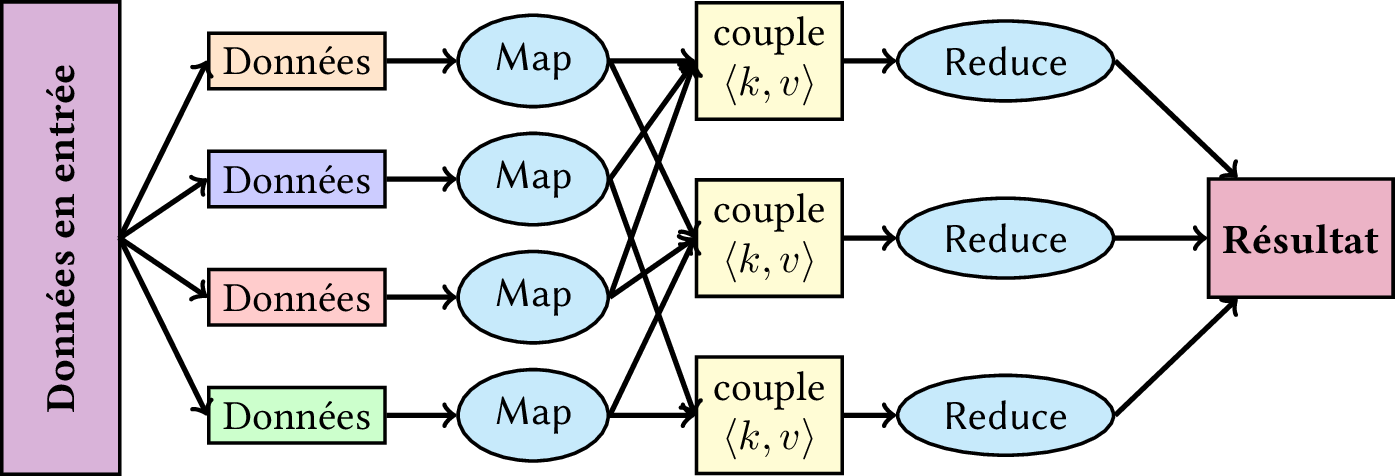
\includegraphics[height=2.7cm]{../images/Mapreduce.png}
\vspace*{-3mm}
\end{center}
}

\visible<2->{
\begin{block}{Un autre bloc}
\begin{itemize}
\item blabla
\item blabla~:
 \begin{itemize}
	\item \textcolor{red}{blablaaaa}
	\item blabla
\end{itemize}
\end{itemize}
\end{block}
}

\visible<3->{
\begin{textblock}{2.5}(-1,-10)
\begin{minipage}{124mm}
\begin{alertblock}{Ne jamais oublier !}
\begin{itemize}
\item Pas plus de 2 minutes par slide
\item Pas trop de textes/figures sur un slide
\item Parlez tranquillement
\item Bougez un peu mais pas trop
\end{itemize}
\end{alertblock}
\end{minipage}
\end{textblock}
}

\end{frame}
\beamerdefaultoverlayspecification{<+->}

%************************** Ajout automatique des plans *****************************
\AtBeginSection[]
{
  \begin{frame}<beamer>
    \ifthenelse{\equal{\TheLanguage}{french}}
 		{\frametitle{Plan}}
 		{\frametitle{Outline}}
    \tableofcontents[currentsection,currentsubsection]
  \end{frame}
  \subsection*{$\empty$} % bidon, pour corriger un bug sur les sous-sections
}

%************************** Part one *******************************************
\section[Partie UN]{Une première partie}
%% *****************************************************************************
% **************            SLIDE
% *****************************************************************************
\beamerdefaultoverlayspecification{}
\begin{frame}[fragile]                           % IL FAUT METTRE FRAGILE A CHAQUE FOIS QU'IL Y A DU CODE A METTRE :(
\frametitle{Un exemple de code}

\vspace*{-1mm}
\begin{block}{Un petit code}                    % Hélas, \visible<1->{   NE FONCTIONNE PAS :(   (pb de compatibilité entre package ...)
\vspace*{-2mm}
\begin{footnotesize}
\begin{java}
public class {
|	...
|	public static void main(String arg){
|	|	System.out.println("sdmklfjsdfj dfsdf ");
|	|	for(int i=0;i<n;i++)
|	|	|	if (1=1)
|	|	|	|	Toto.add(i)
|	}
}
\end{java}
\end{footnotesize}
\vspace*{-2mm}
\end{block}


\vspace*{-1mm}

\visible<2->{
\begin{block}{Commentaires provenant du dossier ShareText}
\begin{itemize}
	\item Citer vos sources~;
	\item Référencer les figures dans le texte~;
	\item Avoir une notation cohérente entre les différents supports~;
	\item Respecter le typographie pour le bien être du relecteur.
\end{itemize}

\end{block}
}

\end{frame}
\beamerdefaultoverlayspecification{<+->}



% *****************************************************************************
% **************            SLIDE
% *****************************************************************************
\beamerdefaultoverlayspecification{}
\begin{frame}[fragile]                           % IL FAUT METTRE FRAGILE A CHAQUE FOIS QU'IL Y A DU CODE A METTRE :(
\frametitle{Un peu de maths}

\visible<1->{
\begin{block}{La formule dans \textcolor{redUPEC}{ShareText}}
\input{../ShareText/maths1.tex}
\end{block}
}

\visible<2->{
\begin{block}{Le tableau dans \textcolor{redUPEC}{ShareText}}
\begin{small}
\begin{tabular}{|l|l|l|}
\hline
Département & Nombre de chaises & Nombre de prises électriques\\
\hline
\hline
ITS & 150 & 20\\
\hline
SI & 149 & 25 \\
\hline
ISBS & 151 & 19\\
\hline
\end{tabular}
\end{small}
\end{block}
}

\visible<3->{
\begin{alertblock}{Théoreme, un résultat très important !}
\[
1+(-1)^n=\begin{cases}
			0, & \text{if $n$ odd}\\
            2, & \text{otherwise}
		 \end{cases}
\]
\end{alertblock}
}

\end{frame}
\beamerdefaultoverlayspecification{<+->}

%************************** Part two *******************************************
\section[Partie DEUX]{Une seconde partie}
%% *****************************************************************************
% **************            SLIDE
% *****************************************************************************
\beamerdefaultoverlayspecification{}
\begin{frame}[fragile]                           % IL FAUT METTRE FRAGILE A CHAQUE FOIS QU'IL Y A DU CODE A METTRE :(
\frametitle{Une courbe}

\begin{center}
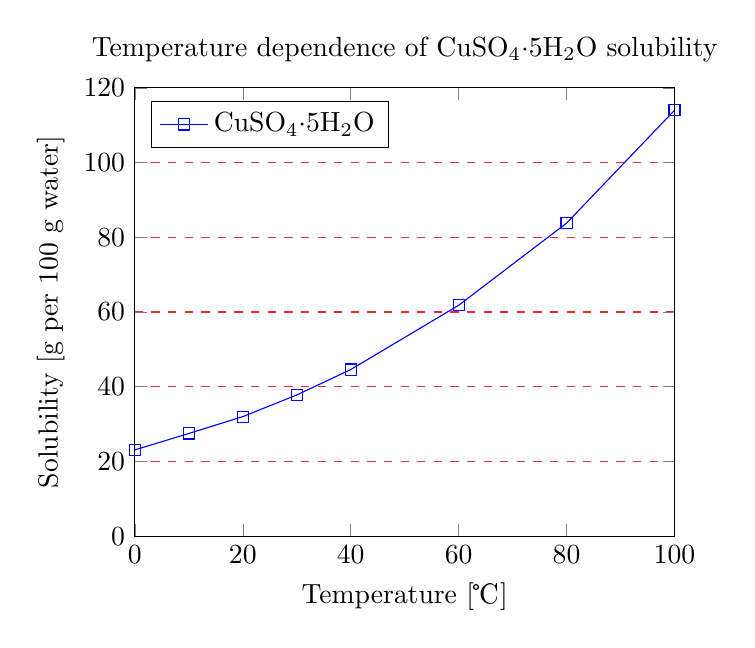
\begin{tikzpicture}
\begin{axis}[
    title={Temperature dependence of CuSO\(_4\cdot\)5H\(_2\)O solubility},
    xlabel={Temperature [\textcelsius]},
    ylabel={Solubility [g per 100 g water]},
    xmin=0, xmax=100,
    ymin=0, ymax=120,
    xtick={0,20,40,60,80,100},
    ytick={0,20,40,60,80,100,120},
    legend pos=north west,
    ymajorgrids=true,
    grid style=dashed,
    grid style={redUPEC},
]
\addplot[
    color=blue,
    mark=square,
    ]
    coordinates {
    (0,23.1)(10,27.5)(20,32)(30,37.8)(40,44.6)(60,61.8)(80,83.8)(100,114)
    };
    \legend{CuSO\(_4\cdot\)5H\(_2\)O}
\end{axis}
\end{tikzpicture}
\end{center}

\end{frame}
\beamerdefaultoverlayspecification{<+->}


% *****************************************************************************
% **************            SLIDE
% *****************************************************************************

% Une petite contrainte
% Si vous souhaitez ajouter du texte avec verbatim, il faut absolument faire une commande comme celle-ci
\defverbatim{\textVerbatimOne}{\begin{verbatim}Vous avez déjà de quoi faire avec tout cela !\end{verbatim}}

\beamerdefaultoverlayspecification{}
\begin{frame}[fragile]                         % IL FAUT METTRE FRAGILE A CHAQUE FOIS QU'IL Y A DU VERBATIM :(
\frametitle{Suite}

\visible<1->{
\begin{block}{Un automate}
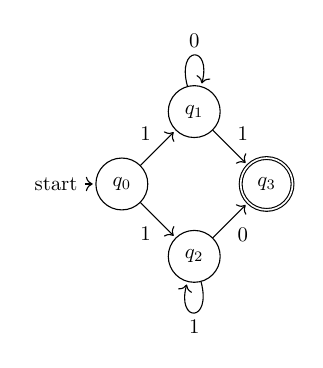
\begin{tikzpicture}[shorten >=1pt,node distance=1.3cm,on grid,auto, every node/.style={scale=0.75}, scale=0.3] 
   \node[state,initial] (q_0)   {$q_0$}; 
   \node[state] (q_1) [above right=of q_0] {$q_1$}; 
   \node[state] (q_2) [below right=of q_0] {$q_2$}; 
   \node[state,accepting](q_3) [below right=of q_1] {$q_3$};
    \path[->] 
    (q_0) edge  node {1} (q_1)
          edge  node [swap] {1} (q_2)
    (q_1) edge  node  {1} (q_3)
          edge [loop above] node {0} ()
    (q_2) edge  node [swap] {0} (q_3) 
          edge [loop below] node {1} ();
\end{tikzpicture}
\end{block}
}

\visible<2->{
\begin{block}{Un texte avec verbatim}
\textVerbatimOne
\end{block}
}

\end{frame}
\beamerdefaultoverlayspecification{<+->}

%************************** Part three *****************************************
\section[Partie TROIS]{Une troisième partie}
%% *****************************************************************************
% **************            SLIDE
% *****************************************************************************
\begin{frame}
\frametitle{Un slide vide}
Allez, au boulot !
\end{frame}

% *****************************************************************************
% **************            SLIDE
% *****************************************************************************
\begin{frame}
\frametitle{Un slide vide}
Allez, au boulot !
\end{frame}

%************************** Conclu ********************************************
\section[Conclusion]{Conclusion}
%% *****************************************************************************
% **************            SLIDE
% *****************************************************************************

\begin{frame}
\frametitle{Pour conclure}

\begin{block}{Ne pas oublier}
\begin{enumerate}
\item De rappeler la problématique
\item Ce qui a été fait
\item Les limitations
\end{enumerate}
\end{block}

\begin{block}{Mais aussi !}
\begin{itemize}
\item Ce qui n'a pas pu être présenté (faute de temps)
\item Ce qui pourrait être amélioré
\item Perspectives, limites, contraintes, {\it etc.}
\end{itemize}
\end{block}

\end{frame}


\plainframe{\Huge \begin{center} \color{redUPEC} Merci ! \\[1cm] Des questions ?  \\ \end{center}}

\end{document}